\documentclass{article}
\title{Intro to PDEs: Ch 5.3 HW}
\author{Logan Rhyne, Harley Combest, Roy Galang, Jesse DiCenso}
\usepackage[T1]{fontenc}
\usepackage{amsfonts, amsmath, amsthm, amssymb}
\usepackage{mathtools, bigints, empheq}
\usepackage{graphicx, wrapfig, xcolor, float}
\usepackage{stackrel}
\usepackage{pgfplots}
\usepackage[shortlabels]{enumitem}
\usepackage[margin=1.0in]{geometry}
\setlength{\parindent}{0pt}
\theoremstyle{definition}
\newtheorem*{lemma}{Lemma}
\newtheorem*{conj}{Conjecture}
\newtheorem{prob}{}
\newtheorem*{pf}{Proof}
\newtheorem*{dpf}{Disproof}
\renewcommand\qedsymbol{$\blacksquare$}
\renewcommand{\emptyset}{\varnothing}
\renewcommand{\epsilon}{\varepsilon}
\newenvironment{disproof}{\begin{proof}[Disproof]}{\end{proof}}
\newenvironment{ans}{\begin{proof}[Answer]\renewcommand{\qedsymbol}{}}{\end{proof}}
\newenvironment{boldenv}{\bfseries\boldmath}{}
\newcommand{\N}{\mathbb{N}}
\newcommand{\Z}{\mathbb{Z}}
\newcommand{\R}{\mathbb{R}}

\pgfplotsset{compat=1.18}

\DeclareMathOperator{\ran}{range}

\begin{document}

\maketitle

\begin{boldenv}
    \underline{Problem 1}. 
    \begin{enumerate}
        \item Consider Dirichlet problem \begin{align}
        & u_{xx} + u_{yy} = 0 \mkern 50mu -\infty < x < \infty, y > 0,\\
        & u|_{y=0} = f(x)
        \end{align}
    Make Fourier transform by $x$, solve problem for ODE for $\hat{u}(k, y)$ which you get as a result and write $u(x,y)$ as a Fourier integral.
        \item Consider Neumann problem \begin{align}
        & u_{xx} + u_{yy} = 0 \mkern 50mu -\infty < x < \infty, y > 0,\\
        & u_y|_{y=0} = f(x)
        \end{align}
    Make Fourier transform by $x$, solve problem for ODE for $\hat{u}(k, y)$ which you get as a result and write $u(x,y)$ as a Fourier integral. What condition must satisfy $f$?
    \end{enumerate}
\end{boldenv}
\begin{ans}
    \begin{enumerate}
        \item \phantom{.}
        \begin{figure}[H]
            \centering
            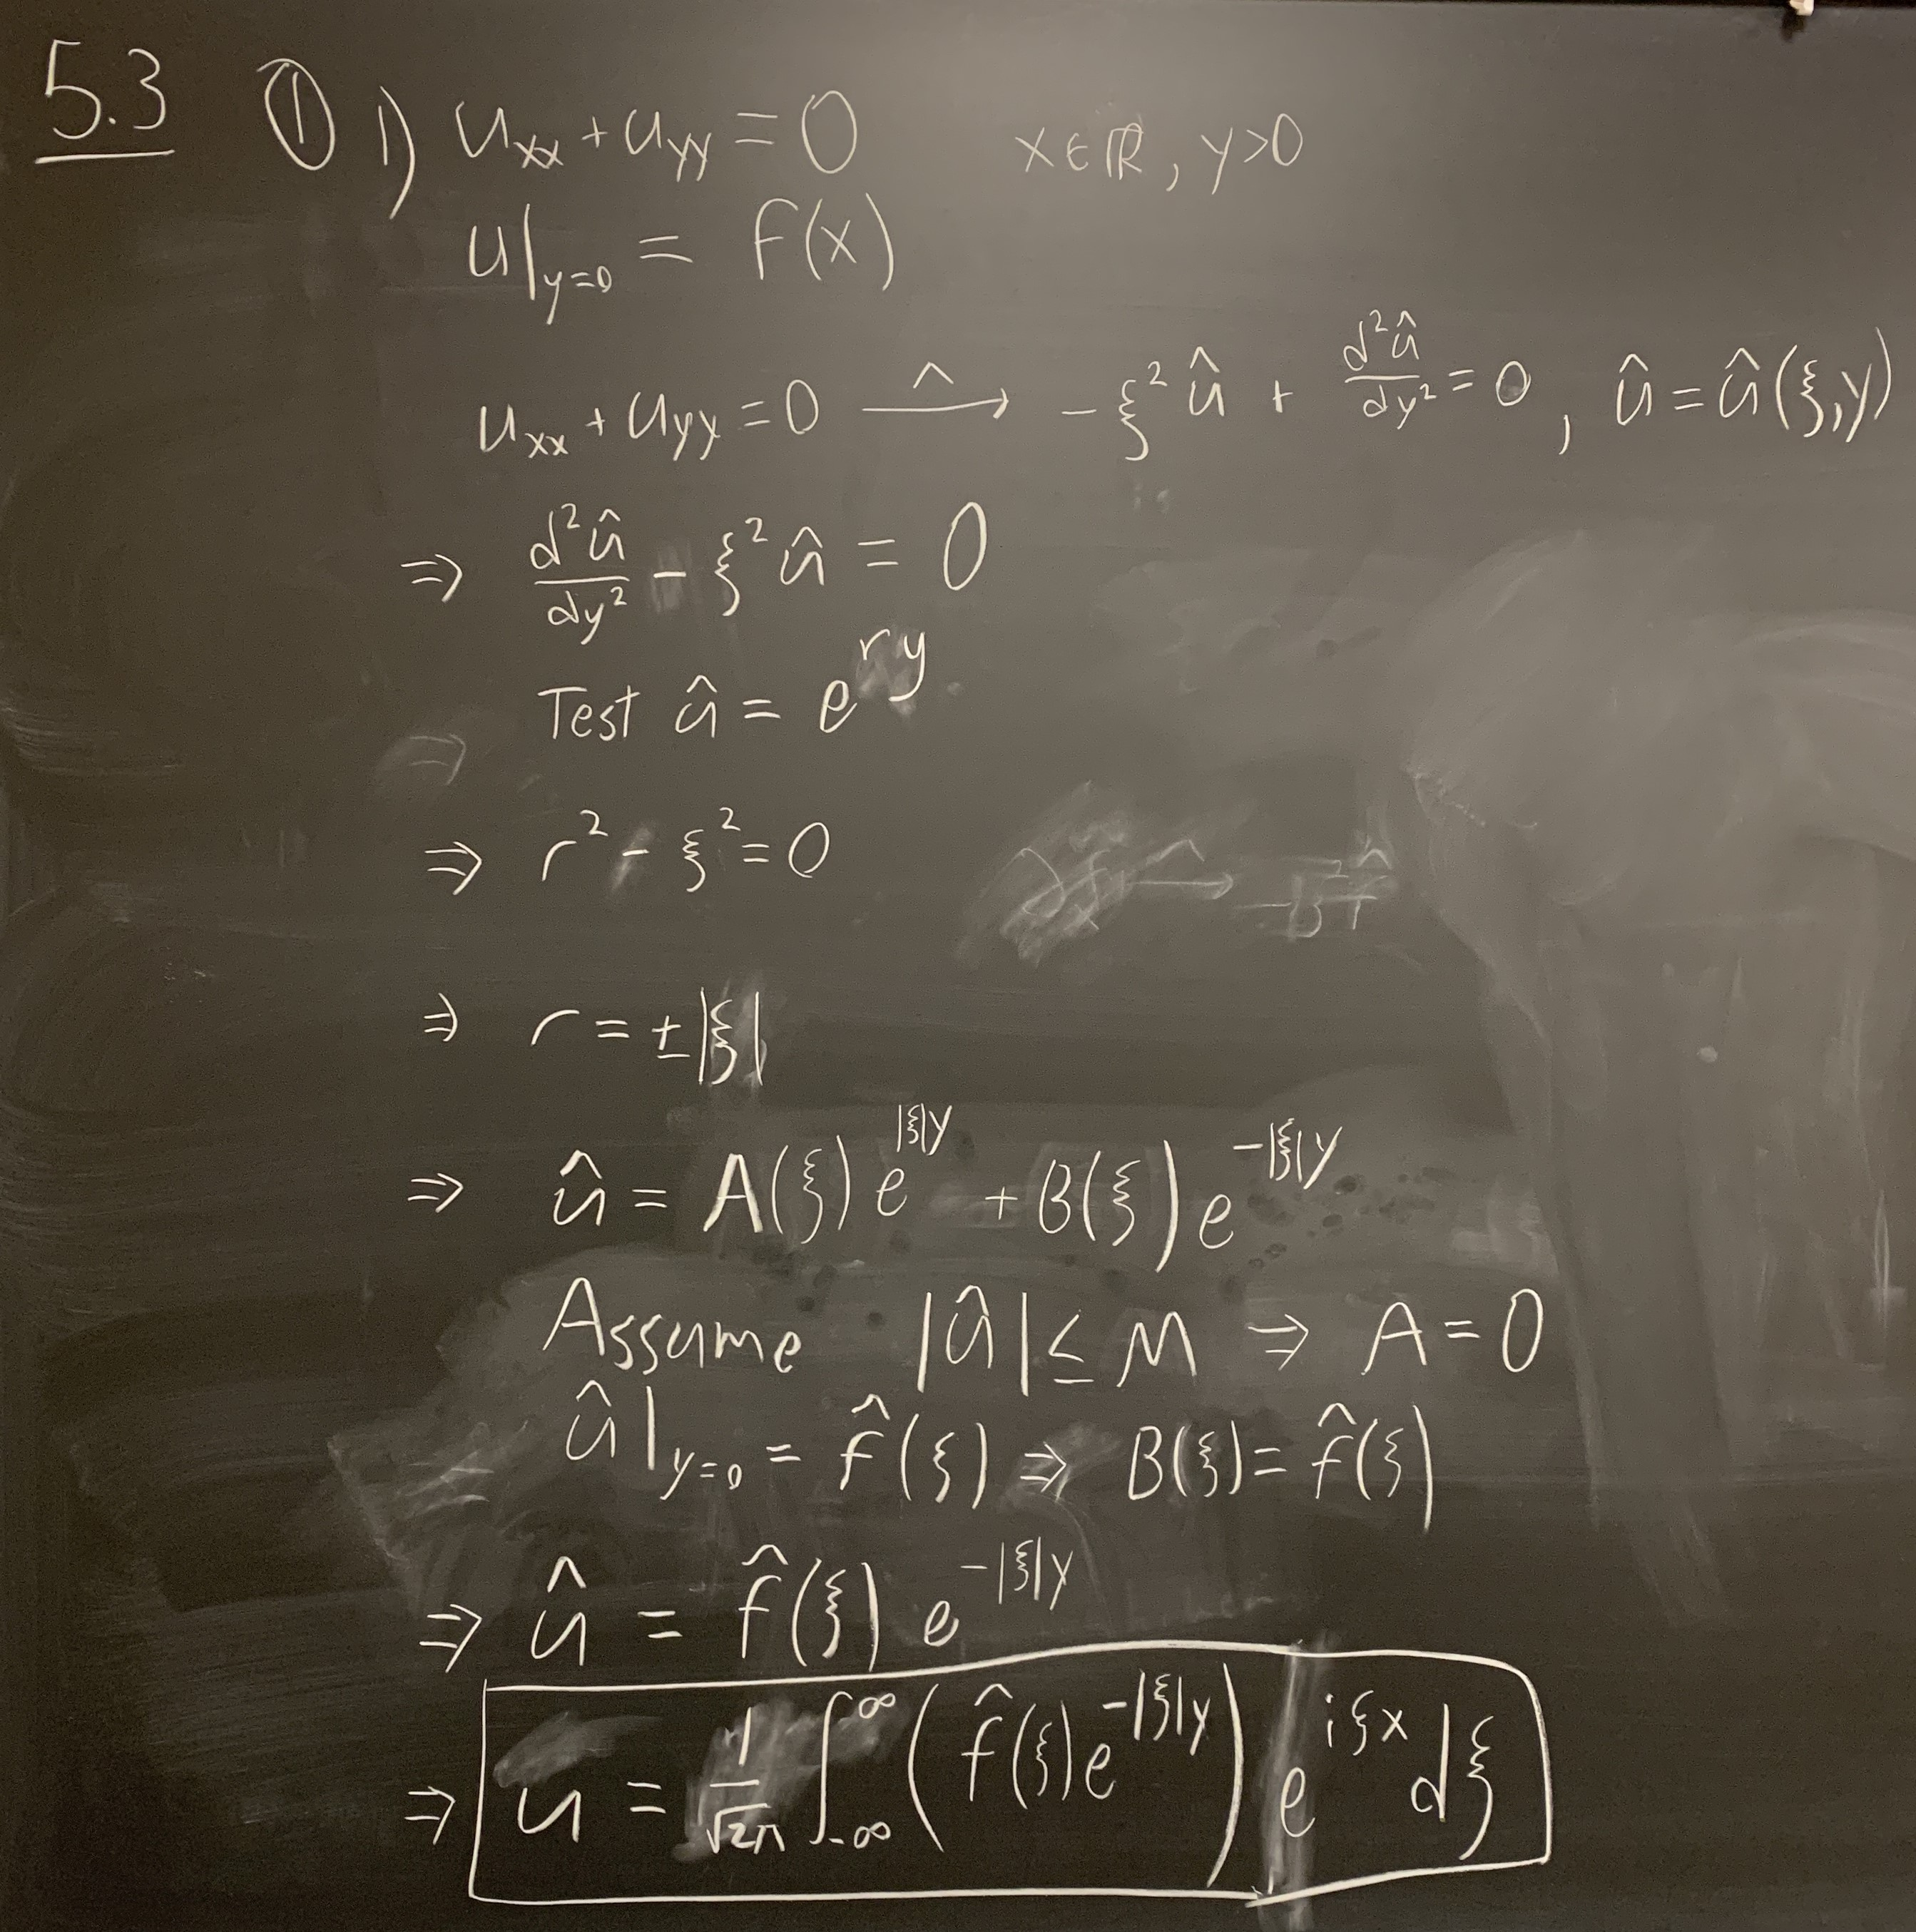
\includegraphics[width = 0.65\textwidth]{Problem 1 part 1.jpeg}
        \end{figure}

        \item \phantom{.}
        \begin{figure}[H]
            \centering
            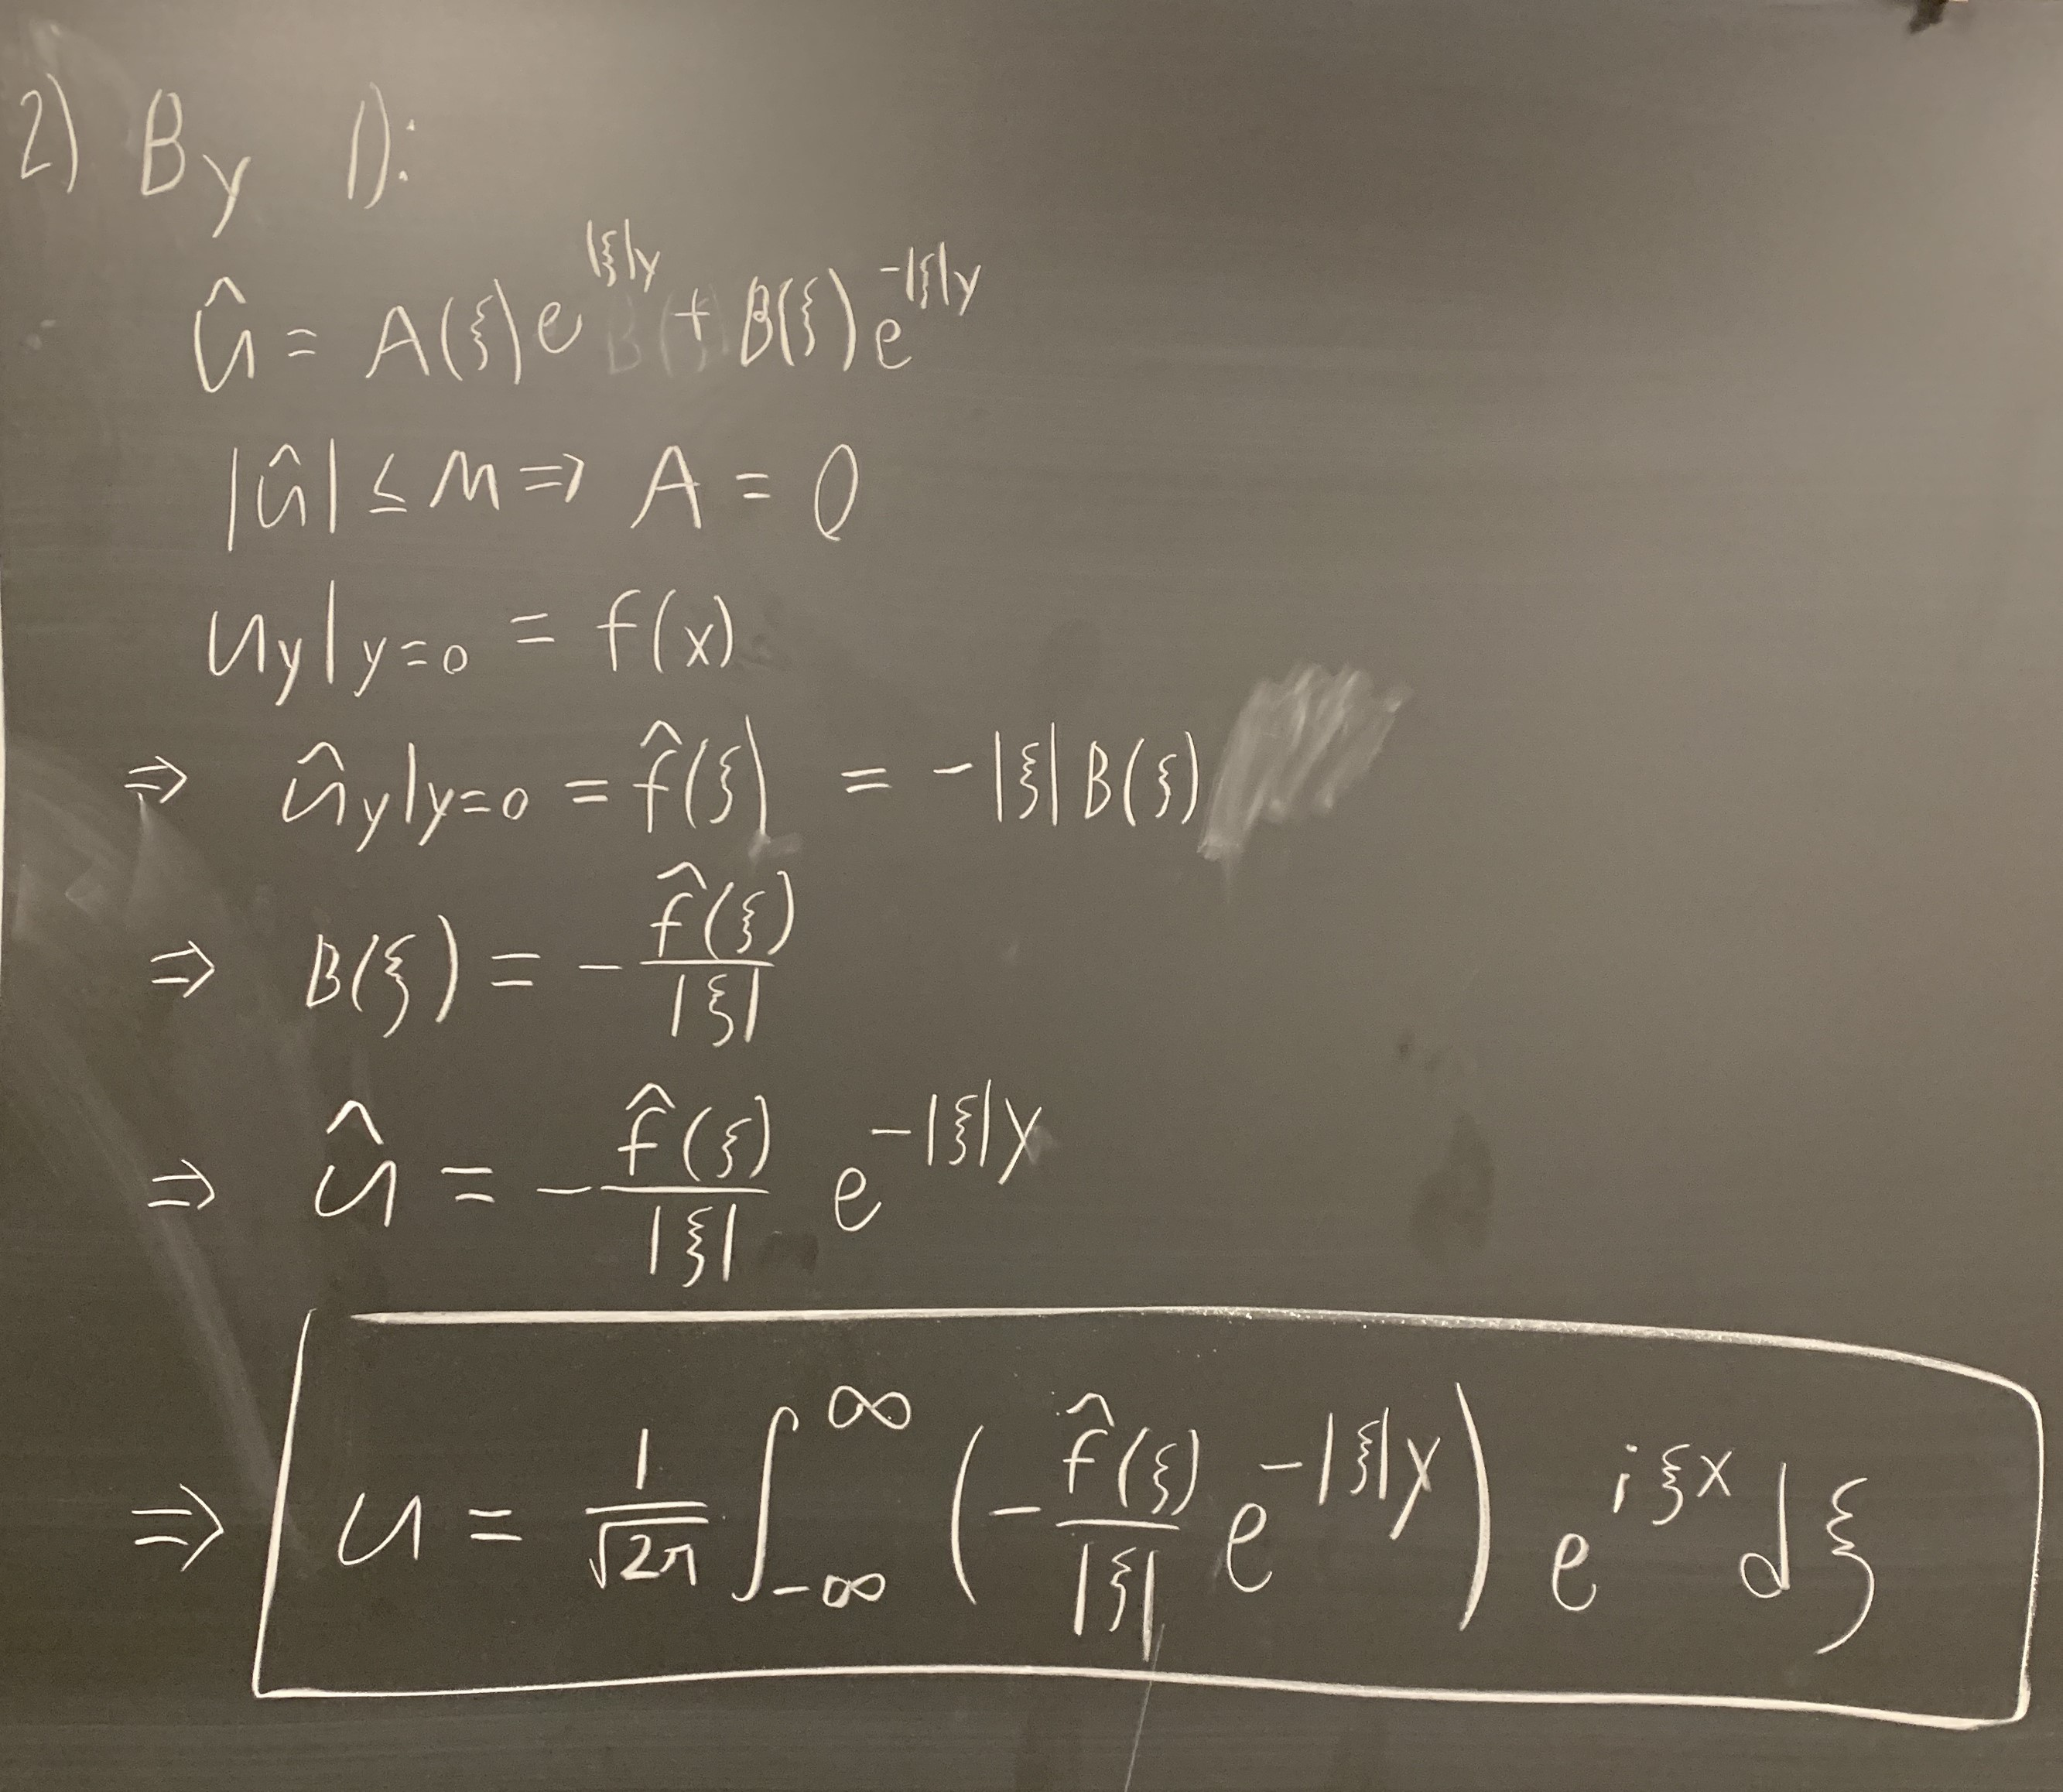
\includegraphics[width = 0.65\textwidth]{Problem 1 part 2.jpeg}
        \end{figure}
    \end{enumerate}
\end{ans}

\begin{boldenv}
    \underline{Problem 2}. 
    \begin{enumerate}
        \item Consider Dirichlet problem \begin{align}
        & u_{xx} + u_{yy} = 0 \mkern 50mu -\infty < x < \infty, 0 < y < 1,\\
        & u|_{y=0} = f(x), \mkern 20mu u|_{y=1} = g(x)
        \end{align}
        Make Fourier transform by $x$, solve problem for ODE for $\hat{u}(k, y)$ which you get as a result and write $u(x,y)$ as a Fourier integral.
        \item Consider Dirichlet-Neumann problem \begin{align}
        & u_{xx} + u_{yy} = 0 \mkern 50mu -\infty < x < \infty, 0 < y < 1,\\
        & u|_{y=0} = f(x), \mkern 20mu u_y|_{y=1} = g(x)
        \end{align}
        Make Fourier transform by $x$, solve problem for ODE for $\hat{u}(k, y)$ which you get as a result and write $u(x,y)$ as a Fourier integral.
        \item Consider Neumann problem \begin{align}
        & u_{xx} + u_{yy} = 0 \mkern 50mu -\infty < x < \infty, 0 < y < 1,\\
        & u_y|_{y=0} = f(x), \mkern 20mu u_y|_{y=1} = g(x)
        \end{align}
        Make Fourier transform by $x$, solve problem for ODE for $\hat{u}(k, y)$ which you get as a result and write $u(x,y)$ as a Fourier integral. What condition must satisfy $f, g$?
    \end{enumerate}
\end{boldenv}
\begin{ans}
    \begin{enumerate}
        \item \phantom{.}
        \begin{figure}[H]
            \centering
            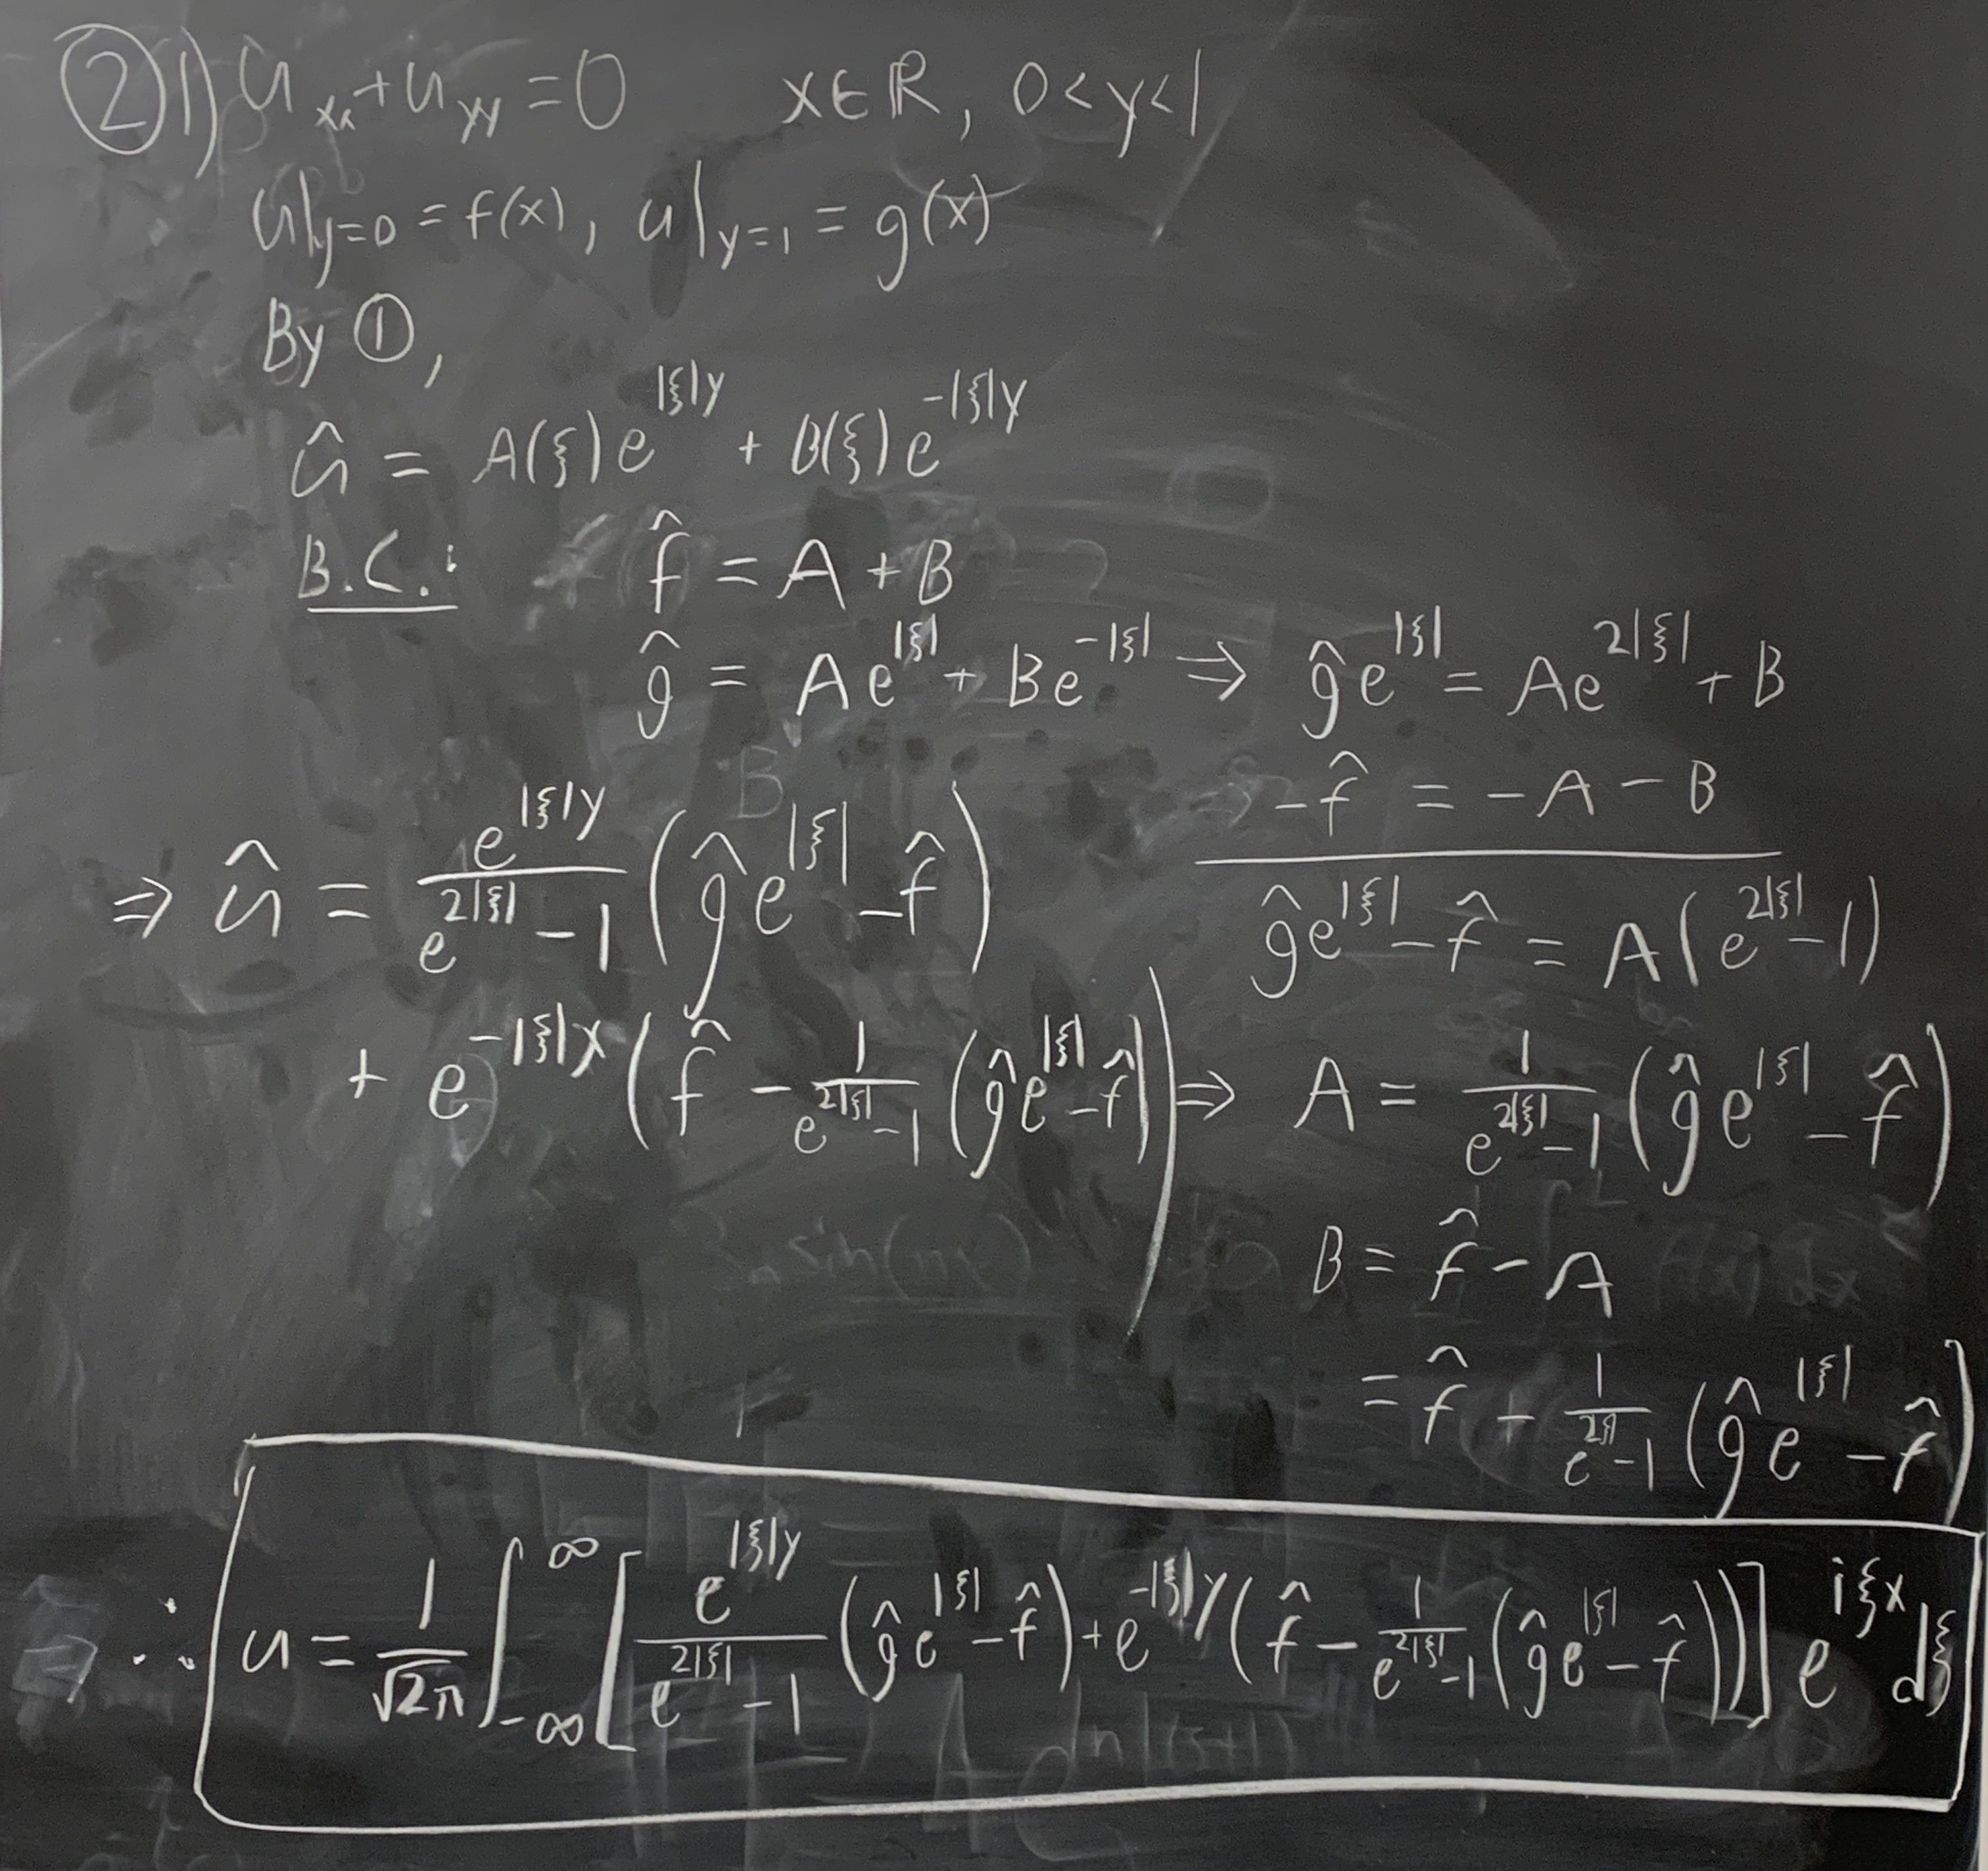
\includegraphics[width = 0.65\textwidth]{Problem 2 Part 1.jpeg}
        \end{figure}

        \item \phantom{.}
        \begin{figure}[H]
            \centering
            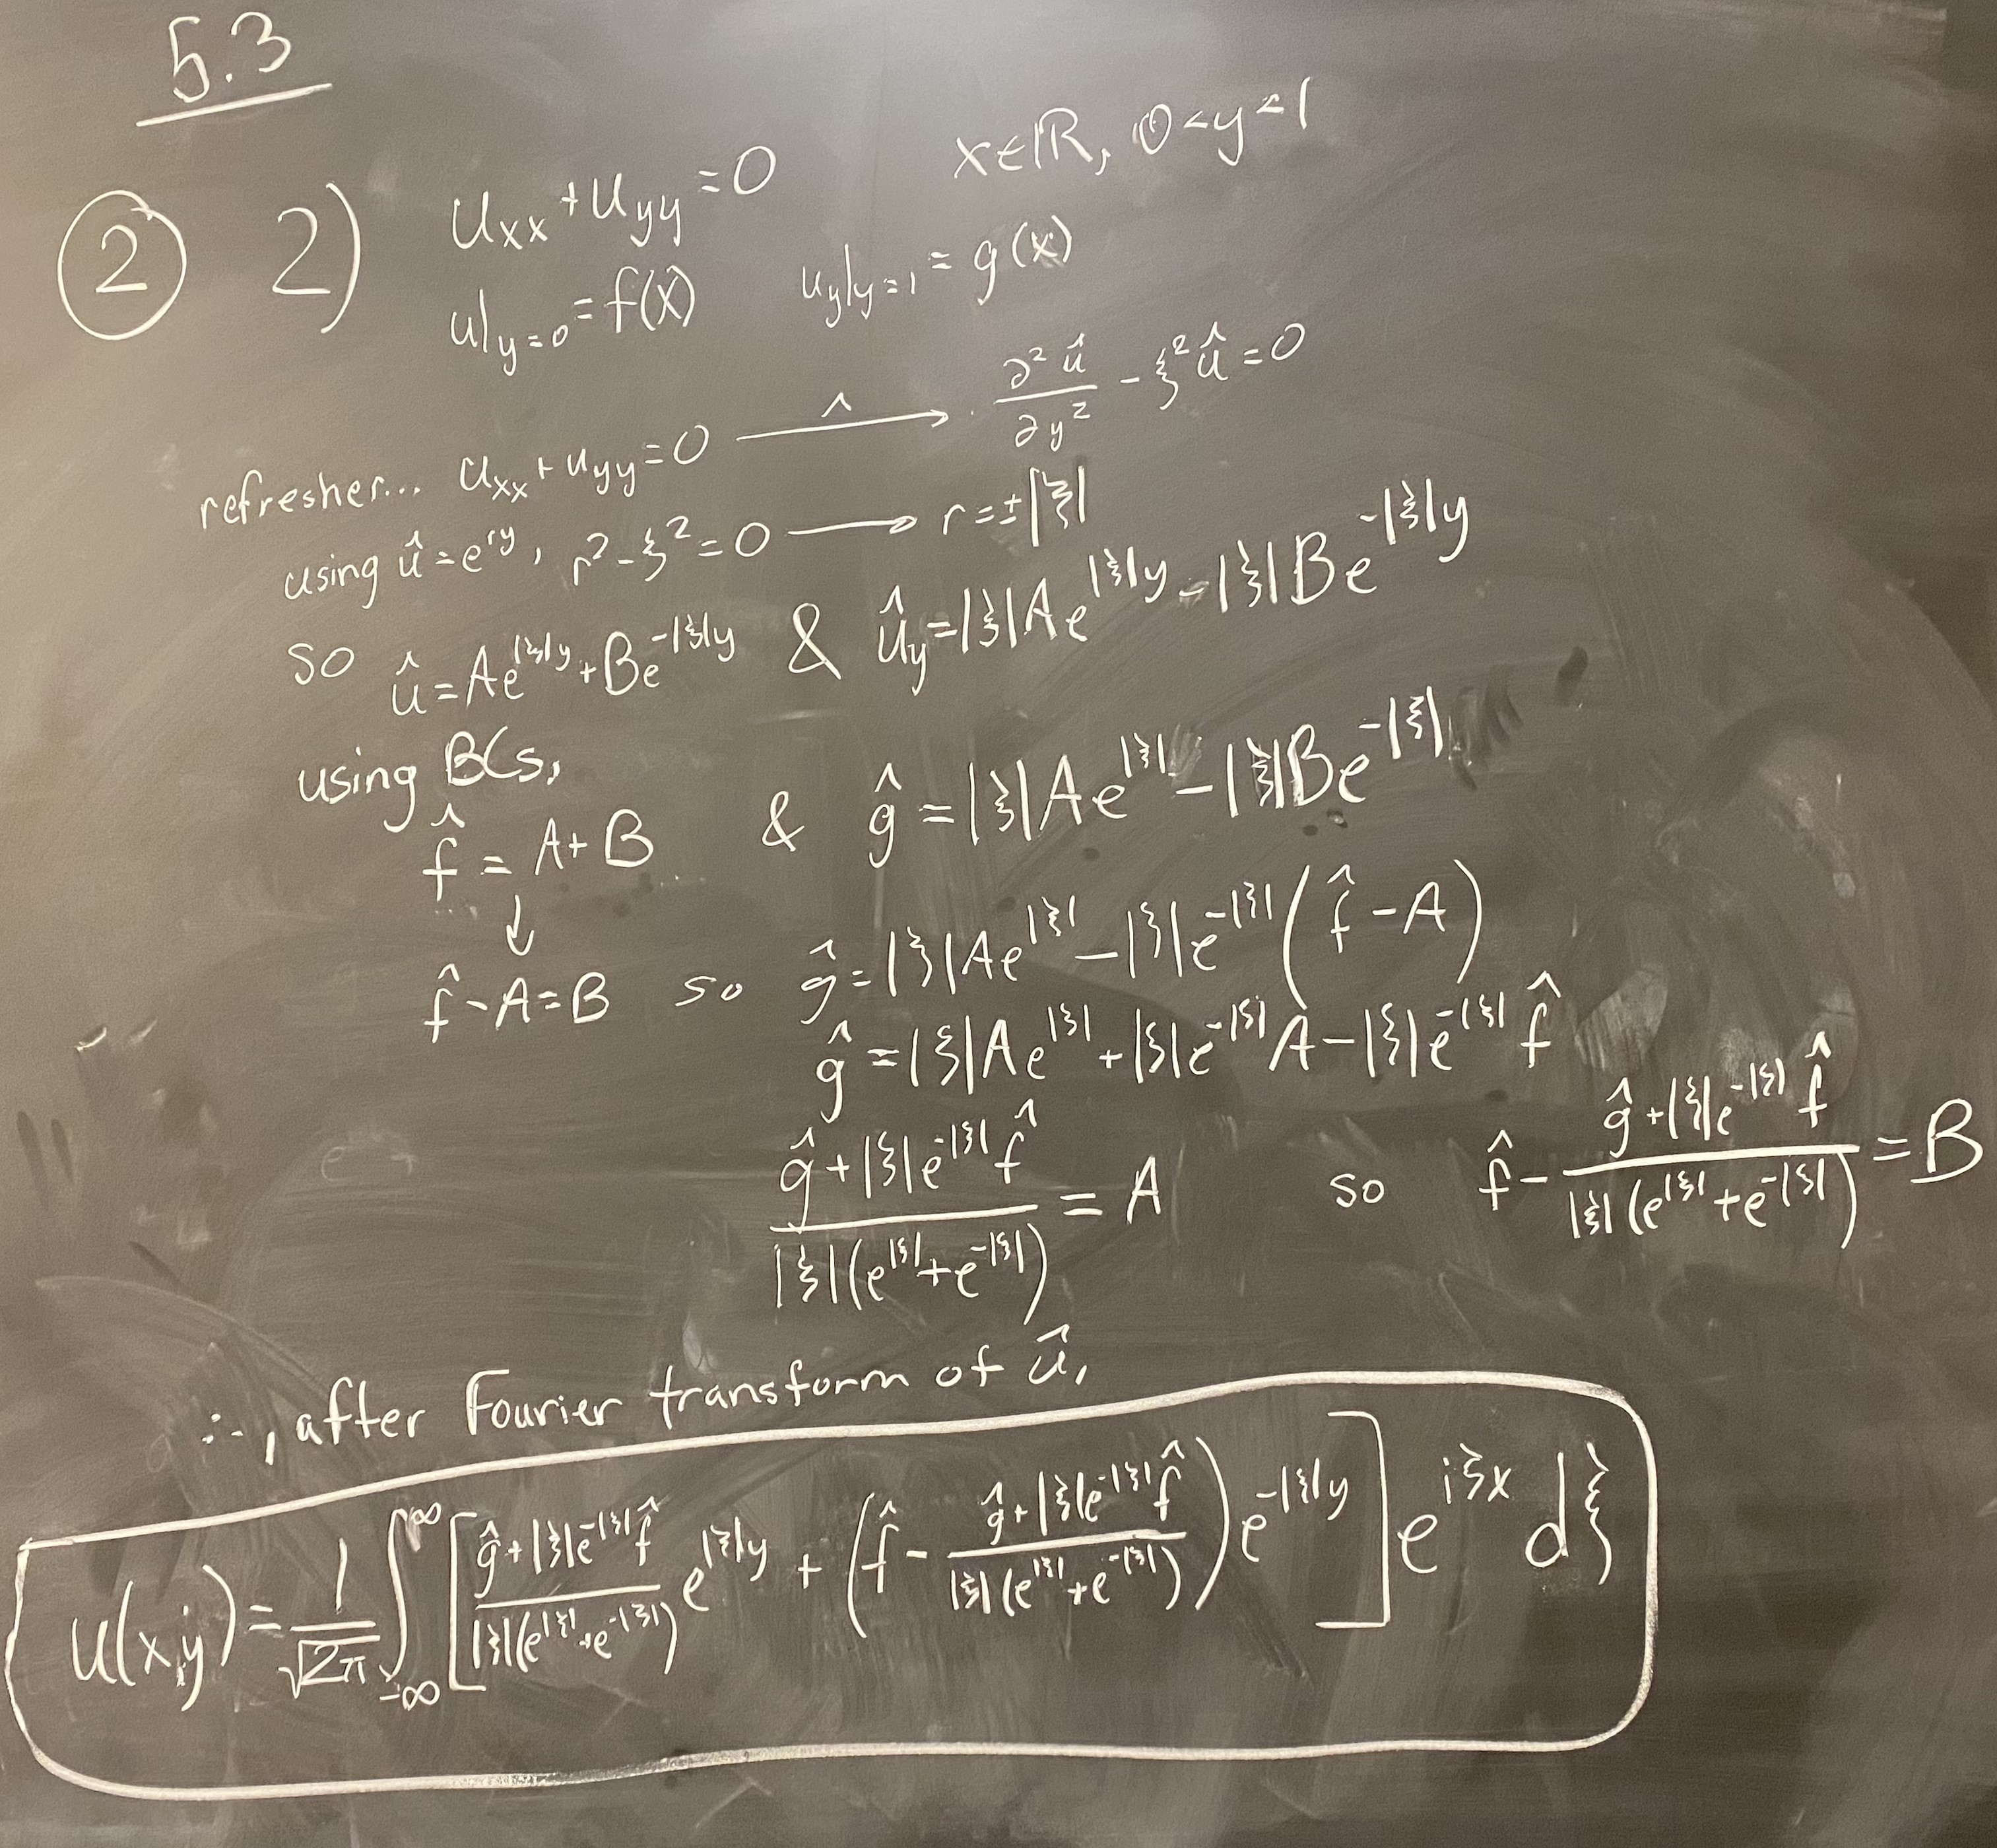
\includegraphics[width = 0.65\textwidth]{Problem 2 Part 2.jpeg}
        \end{figure}

        \item \phantom{.}
        \begin{figure}[H]
            \centering
            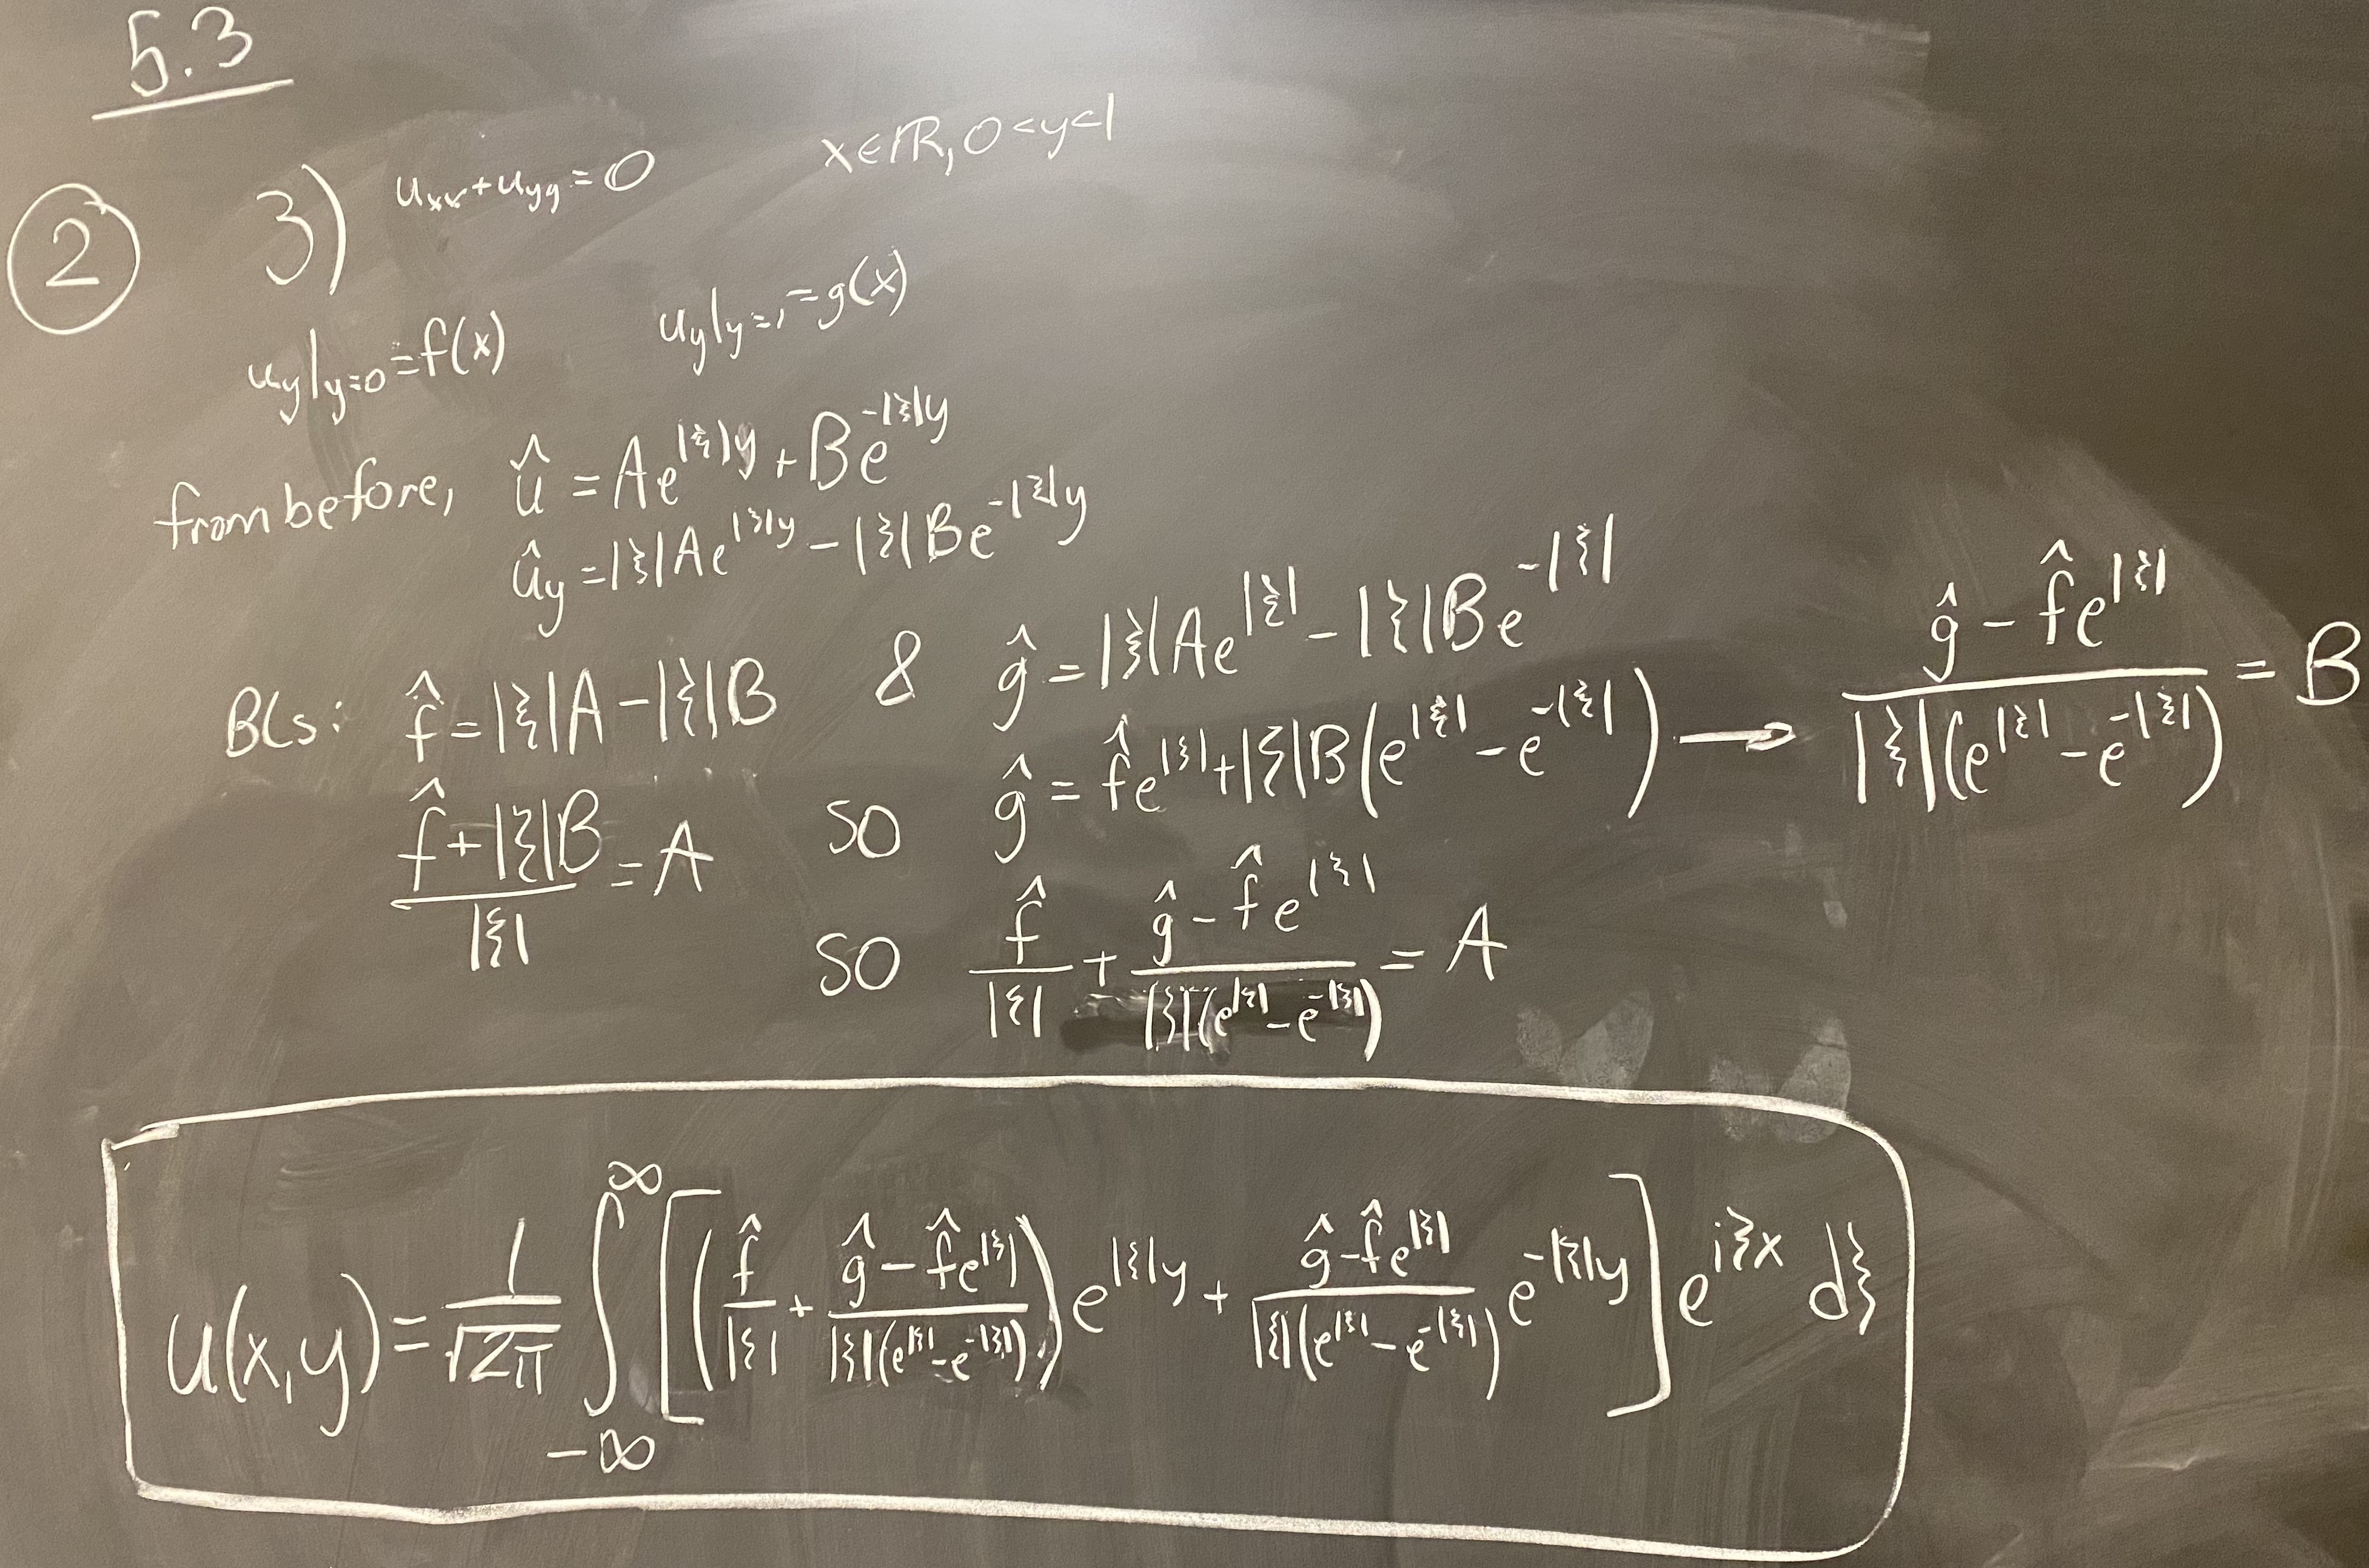
\includegraphics[width = 0.75\textwidth]{Problem 2 Part 3.jpeg}
        \end{figure}
    \end{enumerate}
\end{ans}

\begin{boldenv}
    \underline{Problem 3}. Consider Robin problem \begin{align}
        & u_{xx} + u_{yy} = 0, \mkern 50mu -\infty < x < \infty, y > 0\\
        & (u_y + \alpha u)|_{y=0} = f(x)
    \end{align}
    Make Fourier transform by $x$, solve problem for ODE for $\hat{u}(k, y)$ which you get as a result and write $u(x,y)$ as a Fourier integral. What condition (if any) must satisfy $f$?
    \textit{Hint}. Consider separately cases 
    \begin{align*}
        & \alpha \in \C \backslash \left[0, \infty \right)\\
        & \alpha \in \left[0, \infty \right)
    \end{align*}
\end{boldenv}
\begin{ans}
    \phantom{.}
        \begin{figure}[H]
            \centering
            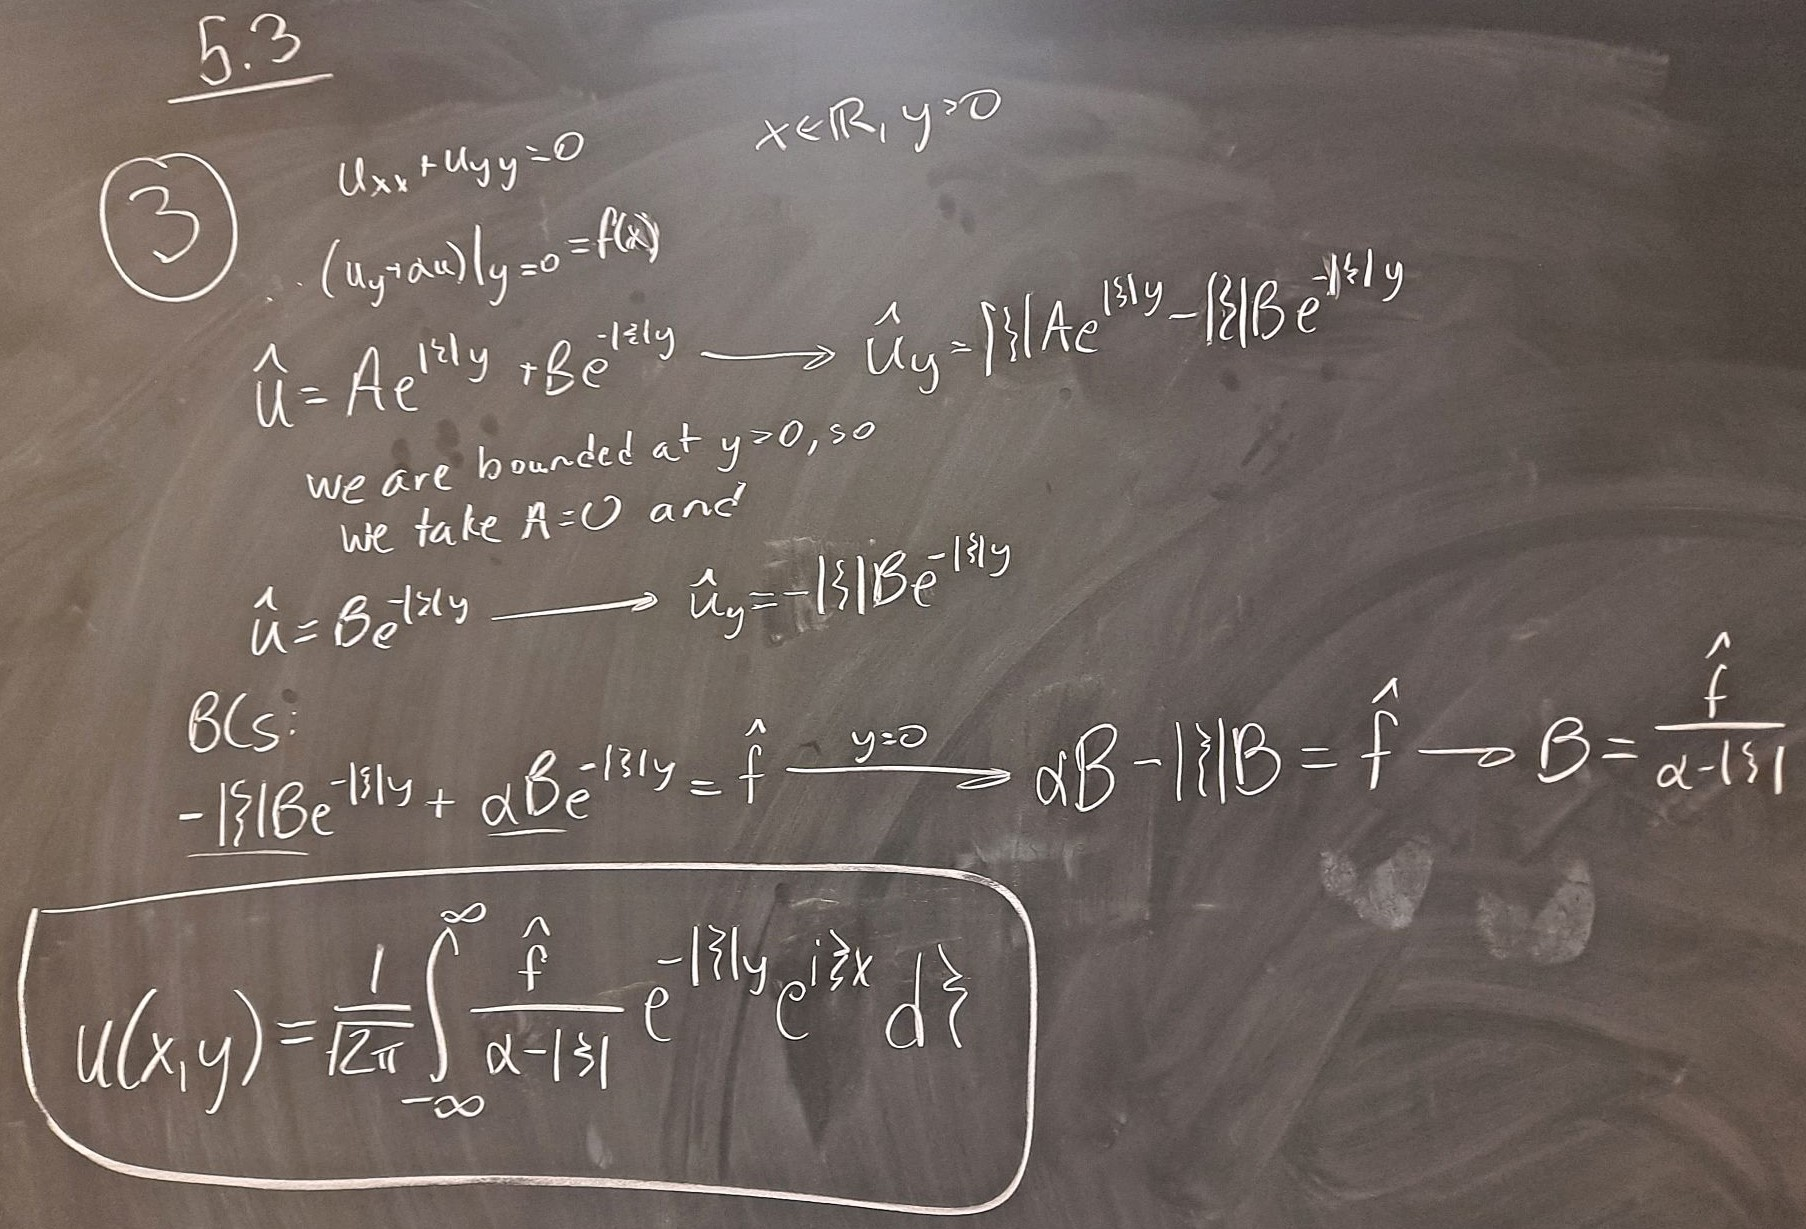
\includegraphics[width = 0.75\textwidth]{Problem 3.jpeg}
        \end{figure}
\end{ans}

\begin{boldenv}
    \underline{Problem 4}.
    \begin{enumerate}
        \item Consider problem \begin{align}
            & \Delta^2u = 0, \mkern 50mu -\infty < x < \infty, y > 0,\\
            & u|_{y=0} = f(x), \mkern 20mu u_y|_{y=0} = g(x)
        \end{align}
        Make Fourier transform by $x$, solve problem for ODE for $\hat{u}(k, y)$ which you get as a result and write $u(x,y)$ as a Fourier integral.
        \item Consider problem \begin{align}
            & \Delta^2u = 0, \mkern 50mu -\infty < x < \infty, y > 0,\\
            & u|_{y=0} = f(x), \mkern 20mu \Delta u|_{y=0} = g(x)
        \end{align}
        Make Fourier transform by $x$, solve problem for ODE for $\hat{u}(k, y)$ which you get as a result and write $u(x,y)$ as a Fourier integral.
        \item Consider problem \begin{align}
            & \Delta^2u = 0, \mkern 50mu -\infty < x < \infty, y > 0,\\
            & \Delta u|_{y=0} = f(x), \mkern 20mu \Delta u_y|_{y=0} = g(x)
        \end{align}
        Make Fourier transform by $x$, solve problem for ODE for $\hat{u}(k, y)$ which you get as a result and write $u(x,y)$ as a Fourier integral. What condition must satisfy $f, g$?
    \end{enumerate}
\end{boldenv}
\begin{ans}
    \begin{enumerate}
        \item \phantom{.}
        \begin{figure}[H]
            \centering
            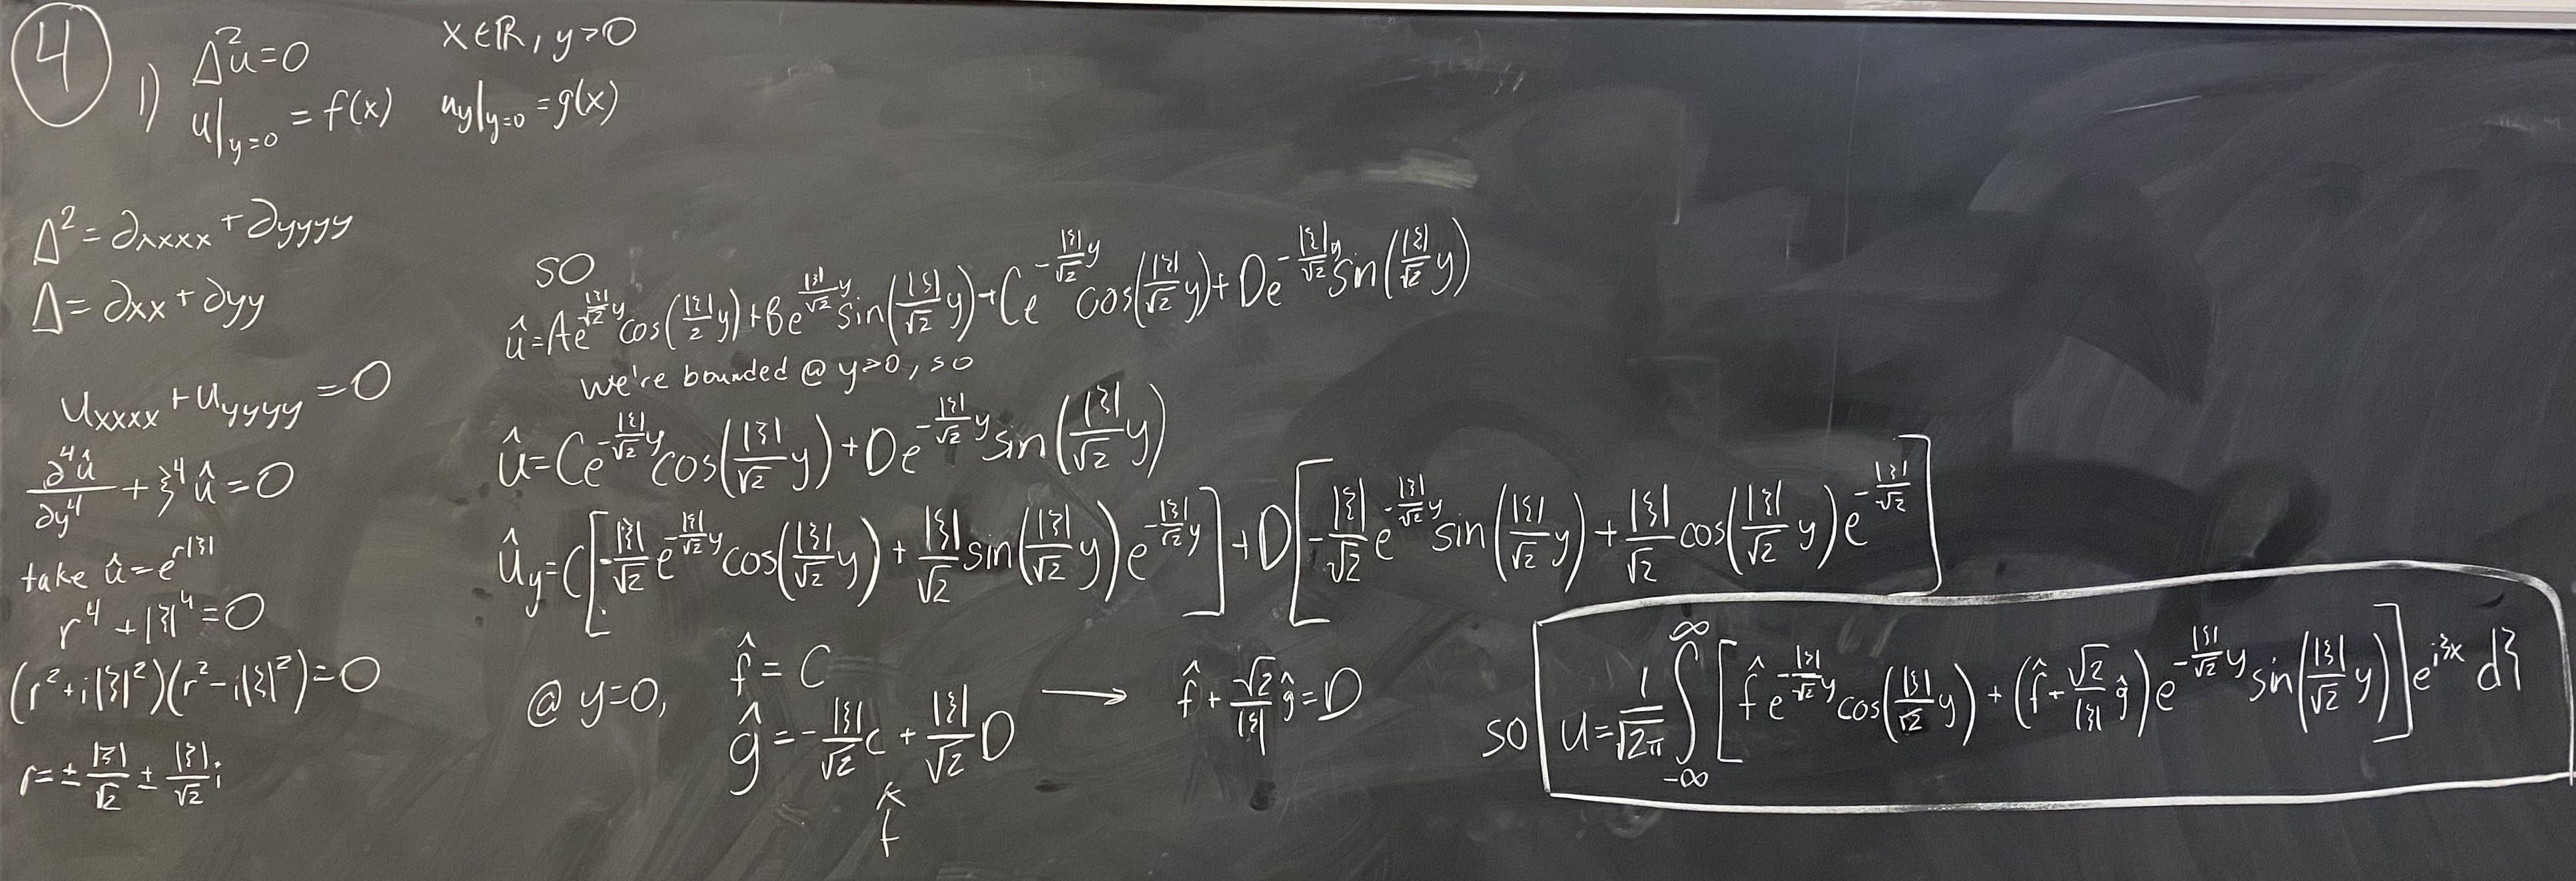
\includegraphics[width = 1\textwidth]{Problem 4 Part 1.jpeg}
        \end{figure}

        \item \phantom{.}
        \begin{figure}[H]
            \centering
            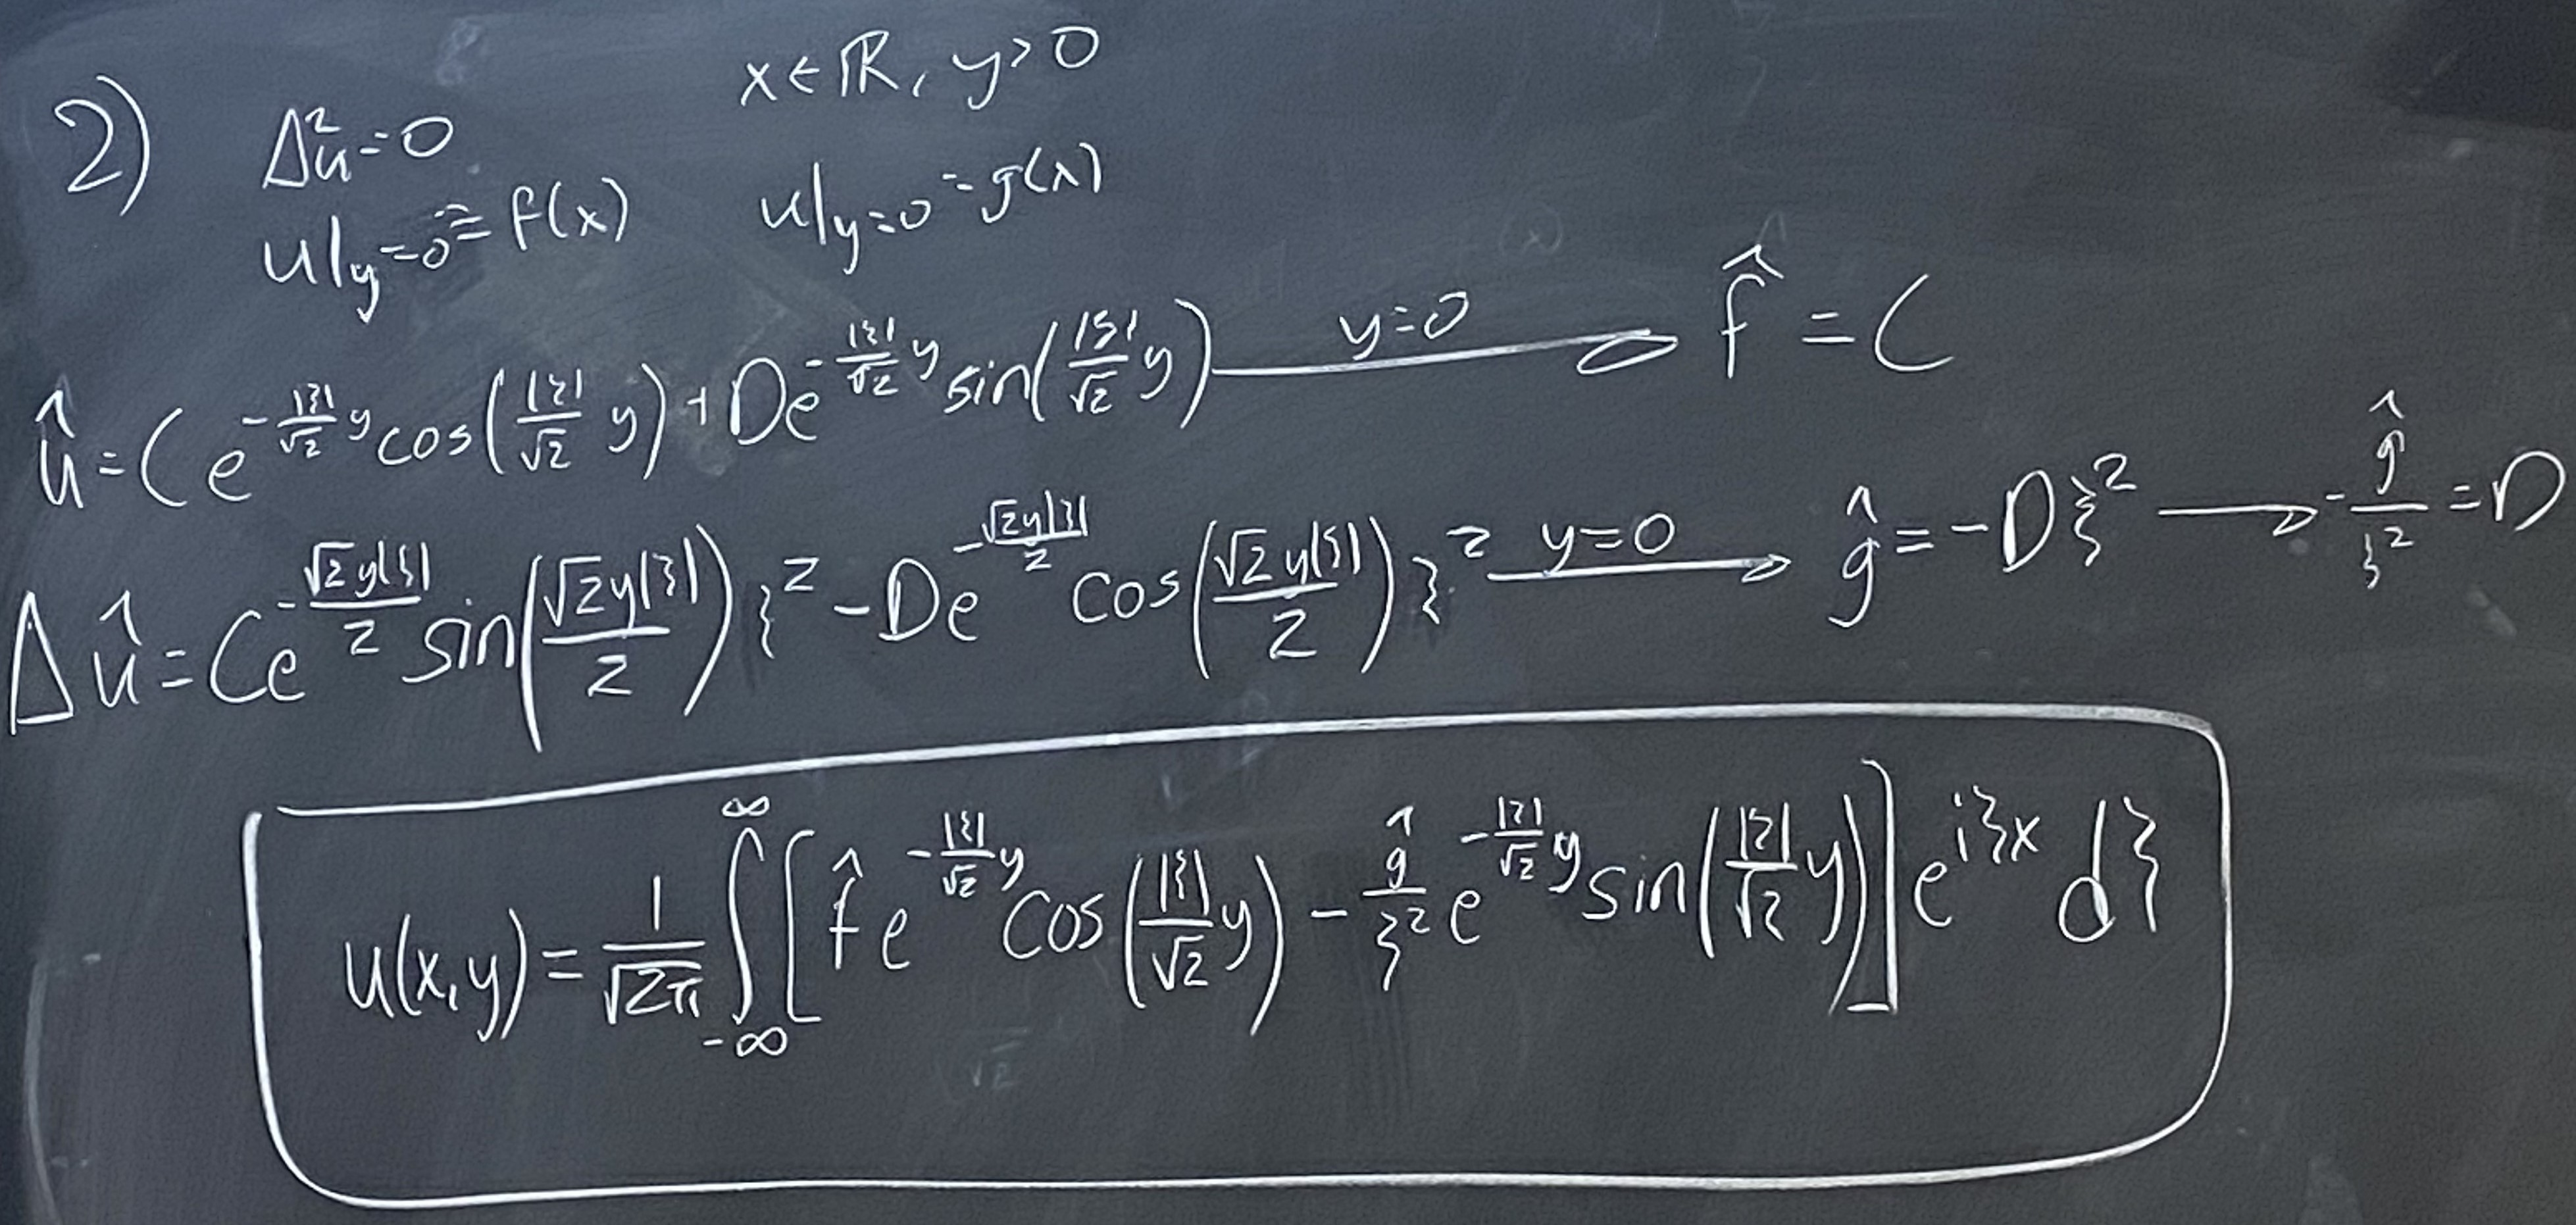
\includegraphics[width = 1\textwidth]{Problem 4 Part 2.jpeg}
        \end{figure}

        \item \phantom{.}
        \begin{figure}[H]
            \centering
            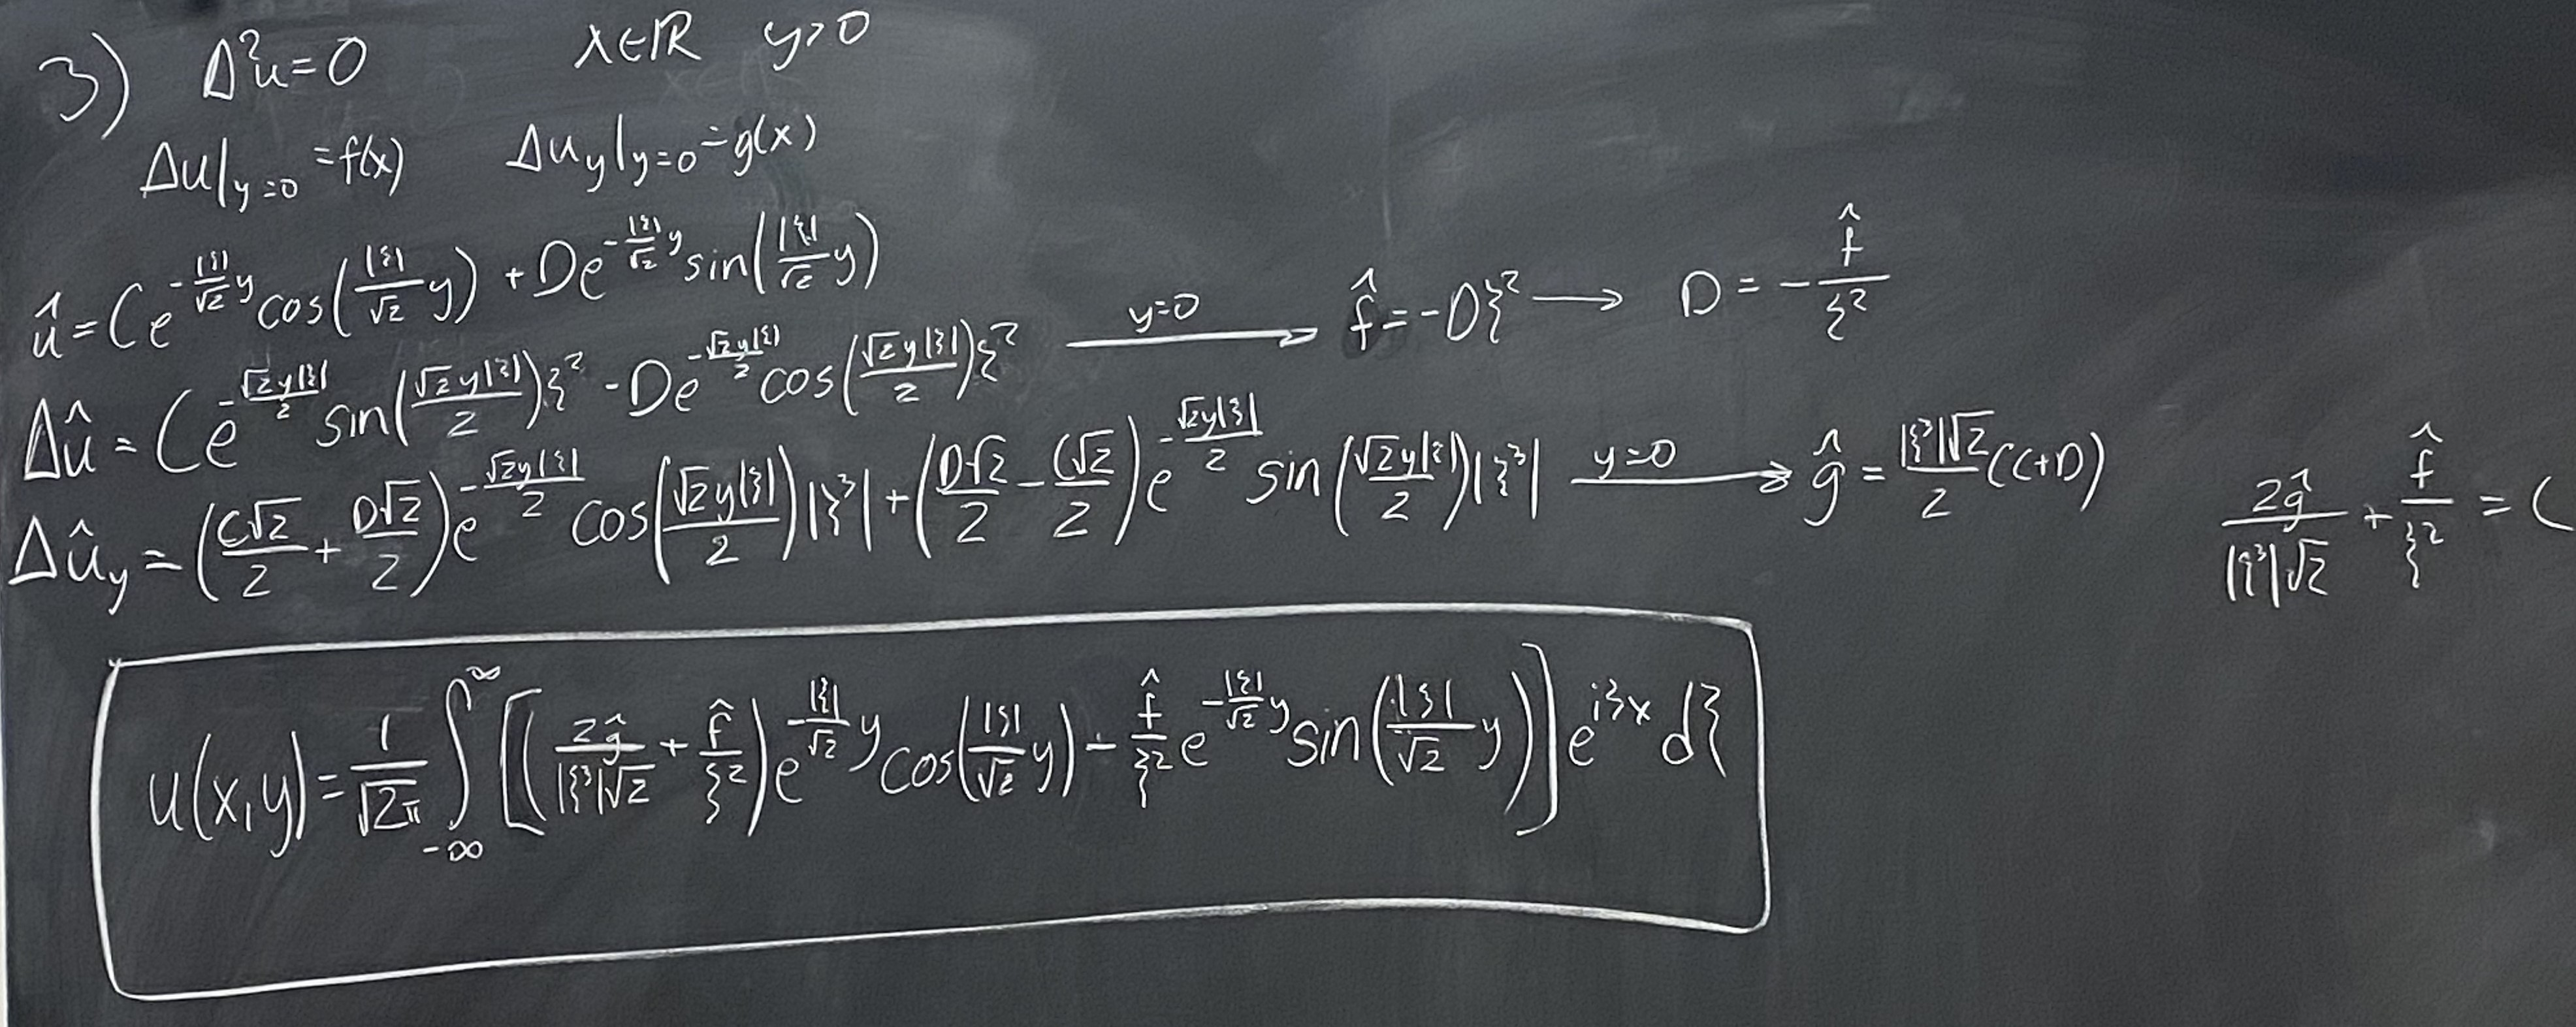
\includegraphics[width = 1\textwidth]{Problem 4 Part 3.jpeg}
        \end{figure}
    \end{enumerate}
\end{ans}

\end{document}
